\chapter{Desenvolvimento}
\label{Desenvolvimento}

A seguir serão abordados os conceitos apresentados previamente a fim de dividir a população em nichos distintos e buscar os melhores indivíduos em cada um deles, explorando bem o espaço de busca e evitando a concentração em somente um máximo ou mínimo local. A estratégia apresentada a seguir tenta resolver o problema evoluindo somente uma população, sem a necessidade de nenhum controle direto sobre a separação dos nichos ou evolução do problema em questão a parte das funções de avaliação e distância.

Esta estratégia é desejável em contextos onde se faz necessária a geração de diversas soluções úteis que não sejam muito semelhantes entre si; contexto muito comum, por exemplo, em jogos com conteúdo gerado proceduralmente, que devem gerar artigos diversificados a fim de evitar repetição e monotonia; comum também em problemas onde a função de avaliação é uma estimativa da solução real, não sendo possível evoluir uma solução direta para o problema, desta forma podemos evoluir soluções variadas que se adaptam bem à função de avaliação e ofereçam uma base para o auxílio à tomada de decisão.

\section{Estratégia de Competição Local}
\label{dev_competicao_local}

A combinação da NS com a estratégia de competição local em um MOEA com eficiência à Pareto, como apresentada em \cite{lehman2011evolving}, provou ser eficiente na busca de diferentes morfologias em um problema de evolução de criaturas virtuais. Isso se deve ao fato da estratégia explorar bem o espaço de busca, identificando nichos com morfologias variadas e mantendo indivíduos com as melhores pontuações dentro de cada nicho. Uma grande vantagem desta estratégia é a capacidade de gerar indivíduos diversificados em uma única execução, enquanto que na maioria dos sistemas de busca evolutiva, descobrir tal diversidade se torna computacionalmente caro; embora execuções diferentes possam resultar em soluções variadas, uma única execução irá tipicamente convergir para somente uma morfologia; além disso, não há garantia de que duas ou mais execuções irão resultar em morfologias diferentes por não haver nenhuma métrica de controle para a diversidade.

Nesta estratégia entretanto, não há nenhuma consideração real em relação à nota de avaliação do indivíduo, sendo utilizada somente a sua nota de competição local e seu valor de dispersão para seleção. Isso implica que nichos que possuem baixas capacidades de performance são mantidos durante a busca, competindo diretamente com indivíduos em nichos com capacidades superiores. No contexto de exploração de nichos esta estratégia é boa, pois mantém os melhores indivíduos de todos os possíveis nichos encontrados; em um contexto onde deseja-se encontrar somente os melhores nichos, contudo, estes indivíduos apenas ocupam espaço na população durante a busca, sem contribuir diretamente para a busca por novos nichos.

\section{Critério Mínimo Global}
\label{dev_criterio_minimo}

A proposta de melhoria oferecida neste trabalho é, portanto, eliminar nichos que possuam uma capacidade funcional muito baixa, evitando que indivíduos destes nichos sejam mantidos por suas notas de competição local. Enquanto possa parecer trivial apenas adicionar a nota de avaliação global como um terceiro objetivo no MOEA, as implicações dessa alteração certamente influenciariam o gradiente de busca, afetando desta forma a procura por novos nichos. O objetivo da melhoria é somente eliminar nichos com notas de avaliação muito baixas, sem influenciar a forma como a busca se espalha pelo espaço das morfologias.

Para endereçar este problema de nichos com baixa capacidade funcional, con\-si\-de\-rou-se a premissa já elaborada em \cite{lehman2010revising} para a MCNS, de que a função crítica para a evolução de qualquer organismo é a habilidade de sobreviver até ser capaz de se reproduzir. Desta forma, esta pesquisa sugere a utilização de um critério mínimo relacionado à função de avaliação global durante o processo de seleção.

Para a introdução deste critério mínimo a implementação escolhida como base foi a PMCNS, pois não necessita da definição de um parâmetro para critério mínimo dependente de domínio e por ser capaz de simular a NS e a MCNS com simples alterações em seus parâmetros de controle. Porém, na implementação aqui proposta, a PMCNS utiliza o critério mínimo de forma diferente, atribuindo zero para a nota de competição local de indivíduos que não atingem o critério mínimo em relação a nota de avaliação global, nunca alterando o valor de inovação calculado. Com isto, devido às características do MOEA, a busca continua a explorar os diversos espaços de morfologias, selecionando e mantendo em sua população somente indivíduos de nichos que atinjam o critério mínimo.

\section{Estratégia de Seleção}
\label{dev_selecao}

Como MOEA para seleção, o algoritmo escolhido para esta pesquisa foi o NSGA-II. Além de rápido e eficiente este também foi o algoritmo utilizado em \cite{lehman2011evolving}, onde teve seu \emph{operador de distância de aglomeração} (${dist}_i$) alterado em prol da diversidade morfológica. A escolha deste algoritmo não só permite uma melhor comparação com os estudos realizados, como também possui este \emph{operador de distância de aglomeração} que pode ser utilizado em favor da busca por diversidade.

O \emph{operador de distância de aglomeração} original ordena os indivíduos dentro de uma frente não dominada de forma que os indivíduos em áreas menos densas tenham maior nota, motivando assim a diversidade dentro de uma mesma frente. No caso onde temos como objetivos a competição local e a diversidade, isso significa que nenhum dos dois objetivos possui vantagem durante a seleção dentro de uma mesma frente somente com base em suas notas. O algoritmo segue escolhendo indivíduos de forma distribuída: tanto indivíduos com alto valor de competição global e baixo valor de diversidade; quanto indivíduos com alto valor de diversidade e baixo valor global; ou qualquer outro indivíduos com trocas de valores equilibradas dentro desta frente possuem chances de ser escolhidas contanto que estejam em áreas menos densas.

A modificação proposta em \cite{lehman2011evolving}, que substitui o \emph{operador de distância de aglomeração}, descrito pela equação \ref{eq:nsgaii_comparacao_de_distribuicao}, por um operador para verificar a diversidade morfológica; passa a ordenar os indivíduos em uma mesma frente de forma a dar preferência a indivíduos com alta diversidade morfológica. Nesta pesquisa, o espaço de busca de morfologias é resultante da função distância definida para o problema; sendo assim, utilizou-se o valor de dispersão (${disp}_i$), calculado conforme a equação \ref{eq:ns_dispersao}, para ordenar os indivíduos dentro de uma mesma frente não dominada, garantindo assim o favorecimento da diversidade morfológica dentro de uma mesma frente não dominada.

Assim sendo, o \emph{novo operador de comparação de distribuição} ($\prec_{n_2}$) é definido pela equação \ref{eq:nsgaii_novo_comparacao_de_distribuicao}
\begin{equation}
    \begin{aligned}
        i\prec_{n_2}j & \quad \quad \text{se }({ranque}_i<{ranque}_j) \\
        & \quad \quad \text{ou } (({ranque}_i={ranque}_j) \text{ e }({disp}_i>{disp}_j)).
    \end{aligned}
    \label{eq:nsgaii_novo_comparacao_de_distribuicao}
\end{equation}

Desta forma o \emph{novo operador de comparação de distribuição} ($\prec_{n_2}$) continua a ordenar indivíduos com base em sua classificação não dominada, mas quando ambas as soluções pertencem à mesma frente, escolhe-se a solução localizada em uma região menos aglomerada em relação ao espaço das morfologias, e não em relação ao espaço dos objetivos. A Figura \ref{fig:dev_selection} é uma representação dos indivíduos selecionados com base na metodologia proposta.

\begin{figure}[htb]
	\begin{center}
		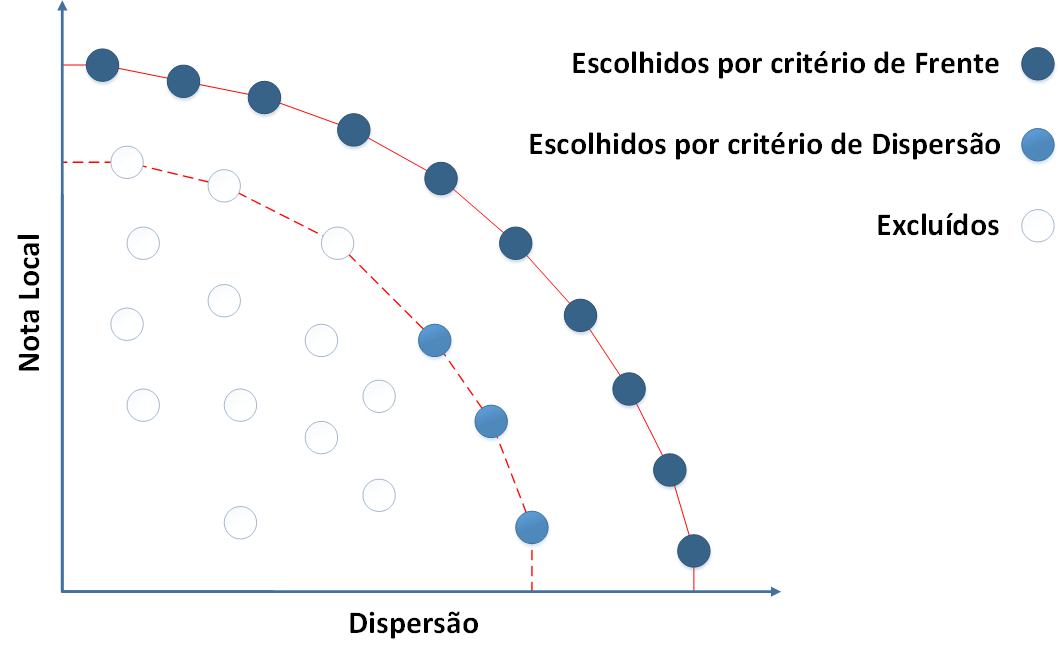
\includegraphics[width=0.8\textwidth]{Imagens/dev_selection.png}
		\caption{Indivíduos em uma mesma frente não dominada são selecionados por critério de Dispersão.}
		\label{fig:dev_selection}
	\end{center}
\end{figure}

\section{Conjunto de Soluções}
\label{dev_conjunto_solucoes}

Com base nas estratégias de competição local e seleção, apresentadas respectivamente nas seções \ref{dev_competicao_local} e \ref{dev_selecao}, o conjunto de soluções final $C_f$ é definido como o conjunto de indivíduos que possuem nota local máxima ao final das execuções. O conjunto $C_f$ representa os indivíduos com maior capacidade funcional dentro de seus próprios nichos, garantindo assim uma boa diversidade entre os resultados. Em um sistema de auxílio à tomada de decisão onde se deve oferecer soluções diversificadas, o conjunto $C_f$ engloba os melhores indivíduos a serem ofertados.

\section{Metodologia Proposta}

A Figura \ref{fig:dev_activity_diagram} apresenta o diagrama de atividades e modificações implementadas para a estratégia elaborada, combinando PMCNS com a utilização de competição local e dispersão como valores objetivos no NSGA-II.

\begin{figure}[htb]
	\begin{center}
		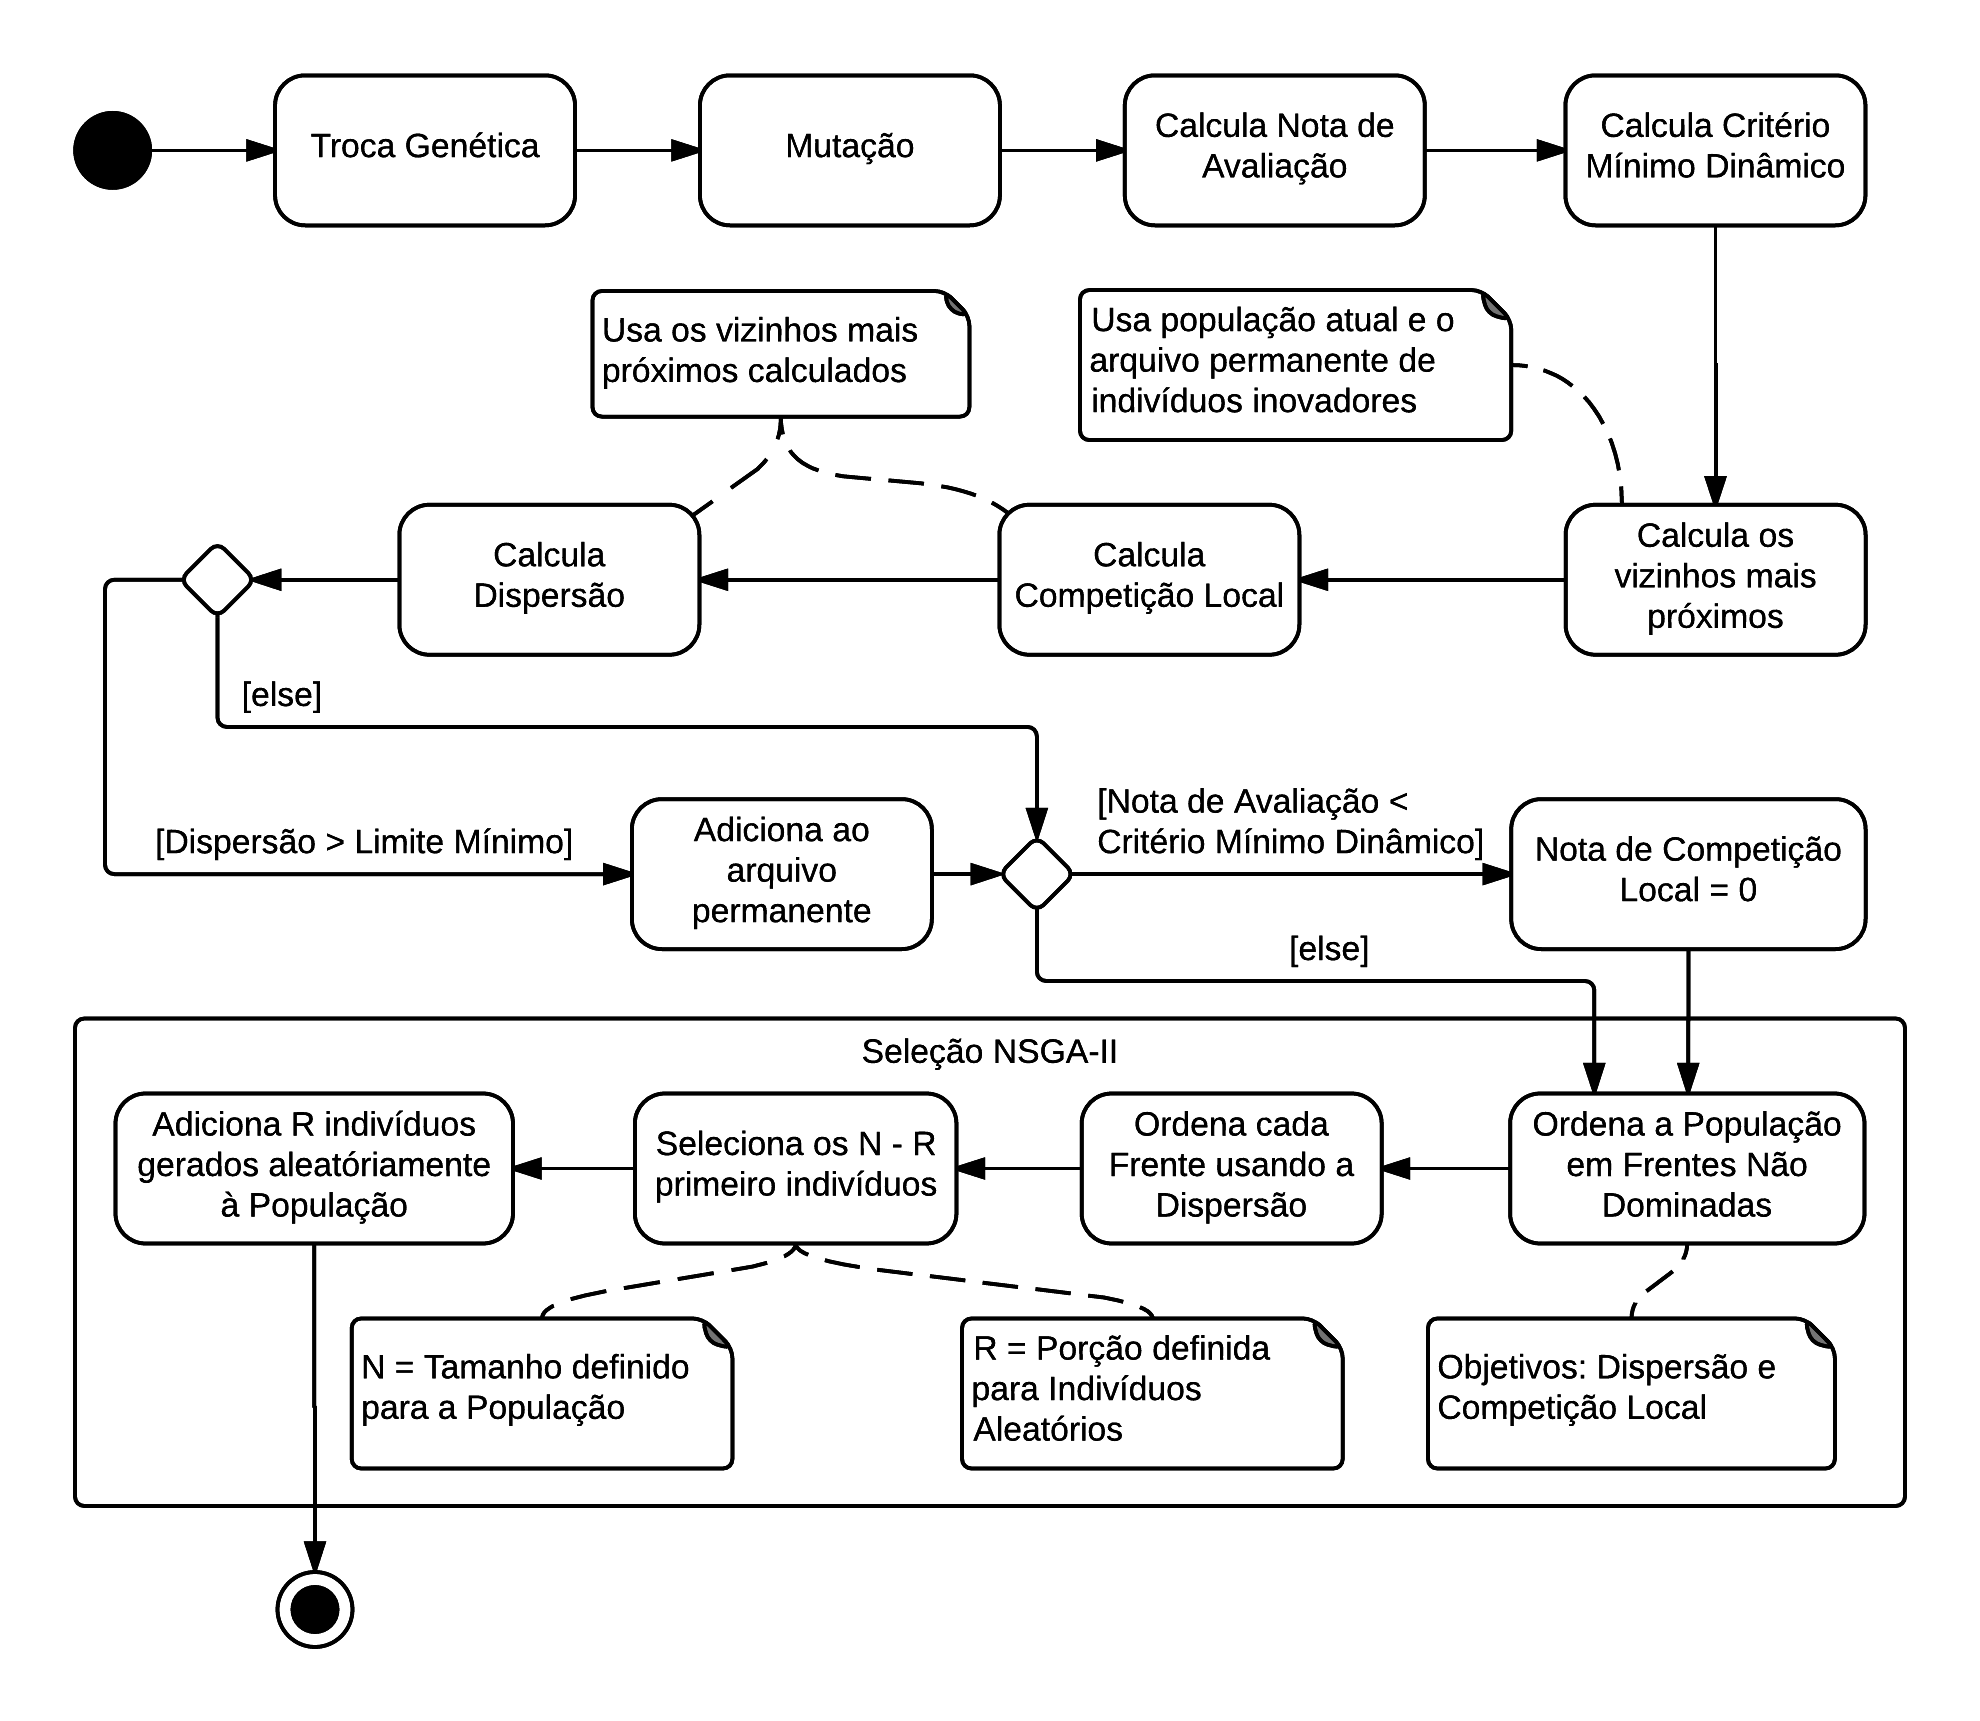
\includegraphics[width=1.0\textwidth]{Imagens/dev_activity_diagram.png}
		\caption{Diagrama de Atividades para o método proposto.}
		\label{fig:dev_activity_diagram}
	\end{center}
\end{figure}

\section{Evoluindo Mapas para um Jogo de Aventura}

Para implementação e testes da técnica proposta, o problema de geração de mapas diferenciados para um jogo de aventura foi o escolhido. Ao gerar novos mapas para um jogo de aventura, buscou-se a criação de mapas que sejam ao mesmo tempo inovadores e interessantes; assim sendo, a estratégia que busca os melhores indivíduos em nichos diferentes se torna promissora para a solução deste tipo de problema.

Um mapa para um jogo de aventura interessante deve apresentar corredores e salas, as quais o jogador deve explorar enquanto combate inimigos e procura a saída para o próximo andar. Para esta pesquisa foram considerados somente o aspecto da exploração do mapa, ignorando quaisquer desafios e obstáculos que possam ser adicionados a um jogo de aventura. Como fator de inovação para os mapas evoluídos, a característica principal analisada foram os aspectos estruturais do mapa, como posicionamento e tamanho das salas e corredores.

\subsection{Representação do Mapa}

Como visto em \cite{cardamone2011evolving}, a representação fenotípica e genotípica dos mapas gerados é um fator importante para a geração automática de conteúdos baseado em busca. A representação deve permitir uma grande variação de conteúdo, ao mesmo tempo que se mantém simples o suficiente para que o algoritmo de busca seja capaz de encontrar indivíduos com boas qualidades.

Os mapas estudados representam uma fase de um jogo de exploração e aventura com visão superior. Sua representação fenotípica é um mapeamento direto da representação do mapa no jogo, definida por uma matriz de dimensões 64 x 64, onde cada entrada representa uma pequena área quadrada do mapa o suficiente para posicionar o personagem do jogador ou qualquer outro elemento, como armadilhas, itens e inimigos. Os possíveis valores para cada entrada na matriz são quatro: vazio, obstáculo, entrada ou saída. As posições vazias do mapa representam corredores e salas, ou seja, áreas por onde o jogador pode navegar livremente, além de possíveis áreas para posicionamento de armadilhas, itens e inimigos. As posições de entrada e saída representam a posição inicial e a posição final para onde o jogador deve caminhar a fim de completar a fase; estas posições devem ser navegáveis entre si. A representação fenotípica foi utilizada para o cálculo de função de avaliação e função de distância. A Figura \ref{fig:dev_phenotype} é a representação de um fenótipo de um mapa com dimensões 16 x 16.

\begin{figure}[htb]
	\begin{center}
		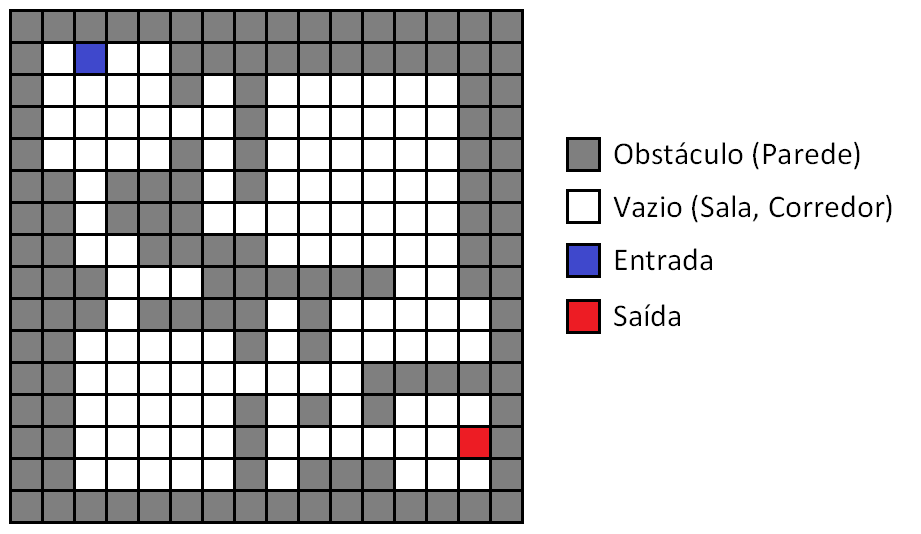
\includegraphics[width=0.7\textwidth]{Imagens/dev_phenotype.png}
		\caption{Representação de um fenótipo de mapa um 16 x 16.}
		\label{fig:dev_phenotype}
	\end{center}
\end{figure}

Como representação genotípica utilizada, optou-se pela representação adotada em \cite{lanzi2014evolving}, uma das propostas de representação apresentadas em \cite{cardamone2011evolving} que gera mapas com espaços reduzidos, característica ideal para um jogo de exploração e aventura. Nesta representação todas as entradas da matriz são, por padrão, obstáculos e somente as entradas vazias são mapeadas de modo a seguir: salas são grandes áreas quadradas do mapa representadas por um terno $<x, y, t>$, onde $x$ e $y$ traduzem a posição central da sala e $t$ o tamanho lateral da arena; de forma semelhante são descritos os corredores, eles são representados por um terno $<x, y, c>$, onde $x$ e $y$ traduzem a posição central do corredor e $c$ traduz tanto o comprimento quanto a direção do corredor (valores positivos representam corredores horizontais e negativos corredores verticais). Em adição a representação original proposta em \cite{cardamone2011evolving}, definiu-se também a entrada e saída, que são representadas por duas duplas $<x, y>$ que traduzem diretamente suas posições no mapa. A figura \ref{fig:dev_genotype} apresenta a estrutura da representação genotípica de um mapa qualquer no sistema.

\begin{figure}[htb]
    \footnotesize
    \sffamily
	\begin{center}
	    \resizebox{\textwidth}{!}{%
            \begin{tabular}{cccc}
                \multicolumn{1}{c|}{Entrada} & \multicolumn{1}{c|}{Saída} & \multicolumn{1}{c|}{Salas} & Corredores \\ \hline
                \multicolumn{1}{c|}{\textless$x_e$, $y_e$\textgreater} & \multicolumn{1}{c|}{\textless$x_s$, $y_s$\textgreater} & \multicolumn{1}{c|}{\textless$x_1$, $y_1$, $l_1$\textgreater … \textless$x_a$, $y_a$, $l_a$\textgreater} & \textless$x_1$, $y_1$, $c_1$\textgreater … \textless$x_b$, $y_b$, $c_b$\textgreater \\
                \multicolumn{4}{c}{} \\
                \multicolumn{4}{c}{e = Entrada, s = Saída, a = Total de Salas, b = Total de Corredores}
            \end{tabular}%
        }
		\caption{Estrutura da representação genotípica de um mapa.}
		\label{fig:dev_genotype}
	\end{center}
\end{figure}

A fim de criar mapas válidos para um jogo de aventura e exploração com o genótipo descrito acima, fez-se necessário a definição de alguns procedimentos adicionais durante a tradução para o fenótipo. Após o posicionamento de todas as salas e corredores, e antes de posicionar a entrada e saída, calcula-se qual é a maior área conexa gerada e removem-se todas as entradas desconexas à esta, fazendo com que voltem a ser consideradas obstáculos. A entrada e saída são posicionadas em seguida, caso estejam em alguma posição considerada como obstáculo são aproximadas através de uma busca radial para a posição vazia mais próxima encontrada. Com estas modificações garante-se que toda a área do mapa é conexa e navegável, certificando a existência de um caminho válido entre a entrada e saída.

Para os experimentos realizados todas as salas possuem tamanho mínimo 10 e máximo 30; os corredores possuem largura 3, comprimento mínimo 3 e máximo 30. Utilizou-se também um número total de 5 salas e 30 corredores, desta forma os mapas gerados possuem algumas grande áreas interligadas por diversos corredores, criando assim um bom ambiente para exploração. Com estas configurações obteve-se, em contraste ao fenótipo de 4096 variáveis, um genótipo final de 109 variáveis (2 para entrada, 2 para saída, 15 para as salas e 90 para os corredores), que possibilita a representação de uma ampla diversidade de mapas ao mesmo tempo permite que o algoritmo de busca encontre indivíduos interessantes.

\subsection{Função de Avaliação}

Naturalmente a escolha da função de avaliação é um fator de extrema importância para o sucesso na execução de algoritmos de busca. Nesta pesquisa, em contraste à outros estudos citados que tentam evoluir mapas interessantes para jogos de tiro \cite{cardamone2011evolving} \cite{lanzi2014evolving} ou estratégia \cite{liapis2013generating} \cite{liapis2013adaptive}, a função de avaliação é montada de forma a incentivar a exploração e aventura do jogador, e por este motivo as posições de entrada e saída são de extrema importância. Os mapas são examinados utilizando uma variação de uma das funções de avaliação proposta em \cite{ashlock2011search}, relativa ao comprimento do menor caminho entre a entrada e saída; quanto mais comprido for o menor caminho existente entre estes, maior o esforço que o jogador precisará realizar a fim de passar para a fase seguinte, contribuindo assim para o fator de exploração e aventura do mapa e fazendo com que ele se torne mais interessante.

Para a função de menor caminho optou-se pelo Algoritmo A*, um algoritmo de busca de menor caminho muito utilizado e conhecido por sua eficiência e precisão. Para a função heurística utilizada escolheu-se a função de Distância de Manhattan, uma vez que os mapas estudados possuem características que se encaixam bem com o uso desta heurística. Permitiu-se também a movimentação nas diagonais no mapa, mas com peso proporcional à diagonal do quadrado; ou seja, o custo de dar um passo na diagonal é maior que o custo de andar na horizontal ou vertical mas ainda é menor que fazer o contorno. Embora permitida a movimentação na diagonal, seguindo o mesmo princípio do paradoxo da conectividade estudado em \cite{resonfeld1966sequential}, não foi permitido que tal movimentação seja possível caso hajam duas paredes nas diagonais adjacentes ao movimento, pois isso implicaria em uma movimentação não muito realista do jogador atravessando algumas paredes. A Figura \ref{fig:dev_movement} mostra as possíveis movimentações do jogador descritas acima.

\begin{figure}[htb]
	\begin{center}
		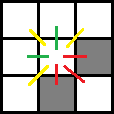
\includegraphics[width=0.2\textwidth]{Imagens/dev_movement.png}
		\caption{Representação das possíveis movimentações do jogador: em verde movimentações com peso normal, em amarelo movimentações com peso maior e em vermelho movimentações não permitidas.}
		\label{fig:dev_movement}
	\end{center}
\end{figure}

O menor caminho representa o mínimo que o jogador deverá explorar até encontrar a saída do mapa, portanto ao utilizar esta métrica que incentiva menores caminhos mais longos, garantiu-se que o jogador precisará explorar e caminhar maiores áreas do mapa, aumentando não somente a área total explorada mas também a quantidade de desafios que irá enfrentar. A Figura \ref{fig:dev_map} representa um mapa com as configurações utilizadas durante os testes e o seu menor caminho.

\begin{figure}[htb]
	\begin{center}
		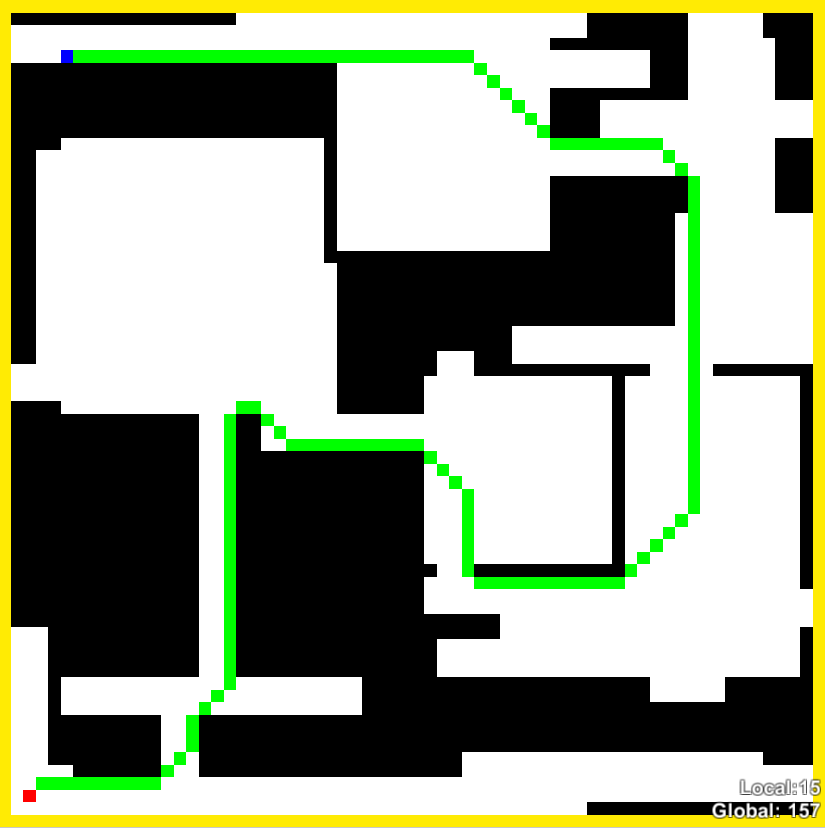
\includegraphics[width=0.6\textwidth]{Imagens/dev_map.png}
		\caption{Mapa obtido com Nota de Avaliação 157.}
		\label{fig:dev_map}
	\end{center}
\end{figure}

\subsection{Função Distância}

Outra função importante a ser definida é a função de distância, esta função é fortemente relacionada ao contexto do problema e normalmente é utilizada na NS para encontrar indivíduos com comportamentos diferenciados. Nesta pesquisa porém, utilizou-se a característica de exploração e busca de indivíduos diferenciados da NS para encontrar mapas distintos, não havendo um comportamento definido que se relacione com a função de avaliação. Além disso, a escolha da função de distância na estratégia escolhida é de extrema importância para a definição do comportamento dos nichos que serão criados durante a busca, uma vez que esta função é utilizada como principal fator de comparação entre os indivíduos. A má escolha de uma função de distância pode resultar em agrupamentos com características não relevantes ao objetivo, portanto a escolha de uma boa função de distância é crucial para o bom funcionamento da estratégia aplicada.

Para o problema de evolução de mapas em questão, a função de distância definida compara indivíduos estruturalmente diferentes; considerando, por exemplo, posicionamento e tamanho das salas e corredores. Para esta comparação utilizou-se um cálculo de distância puramente fenotípica, uma vez que esta representação está diretamente relacionada às características estruturais finais do mapa.

O cálculo de distância fenotípica é a comparação direta entre o fenótipo dos mapas em questão; ou seja, compara-se diretamente cada uma das 4096 variáveis do fenótipo de dois mapas e tem-se como distância final o número de comparações diferentes entre eles. Desta forma, quando mapas muito parecidos são comparados um baixo valor de distância é obtido, uma vez que muitas de suas variáveis coincidem; de forma oposta, quando mapas com áreas abertas em locais diferentes são comparados o valor de distância calculado é grande.

O valor de diferença entre dois valores $x$ e $y$ quaisquer contidos na matriz de fenótipo de um mapa é dada pela equação \ref{eq:dif}

\begin{equation}
    \begin{aligned}
        dif(x,y) = \begin{cases}0 & x = y\\1 & x \neq y\end{cases}
    \end{aligned}~.
    \label{eq:dif}
\end{equation}

Sendo assim, a distância final entre dois mapas é calculado pela equação \ref{eq:dist}

\begin{equation}
    \begin{aligned}
        dist(A,B) = \sum_{i=0}^m\sum_{j=0}^ndif(A_{ij}, B_{ij}),
    \end{aligned}
    \label{eq:dist}
\end{equation}

\noindent onde A e B são as matrizes de representação do fenótipo de dois mapas distintos e $dif(A_{ij}, B_{ij})$ é o valor de diferença da mesma posição nas duas matrizes calculado de acordo com a equação \ref{eq:dif}.

Devido a natureza da NS, que exige que as distâncias entre todos os elementos da população sejam recalculadas em todas as épocas, este cálculo, embora simples, é um dos grandes gargalos de eficiência do algoritmo, por isso optou-se por realizar todos os cálculos relacionados a distância em \emph{threads} paralelas, otimizando assim a utilização dos núcleos da máquina para o mesmo.

\section{Diagrama de Classes}

A Figura \ref{fig:dev_class_diagram} a seguir apresenta o diagrama de classes do pacote computacional desenvolvido para esta pesquisa.

\begin{figure}[htb]
	\begin{center}
		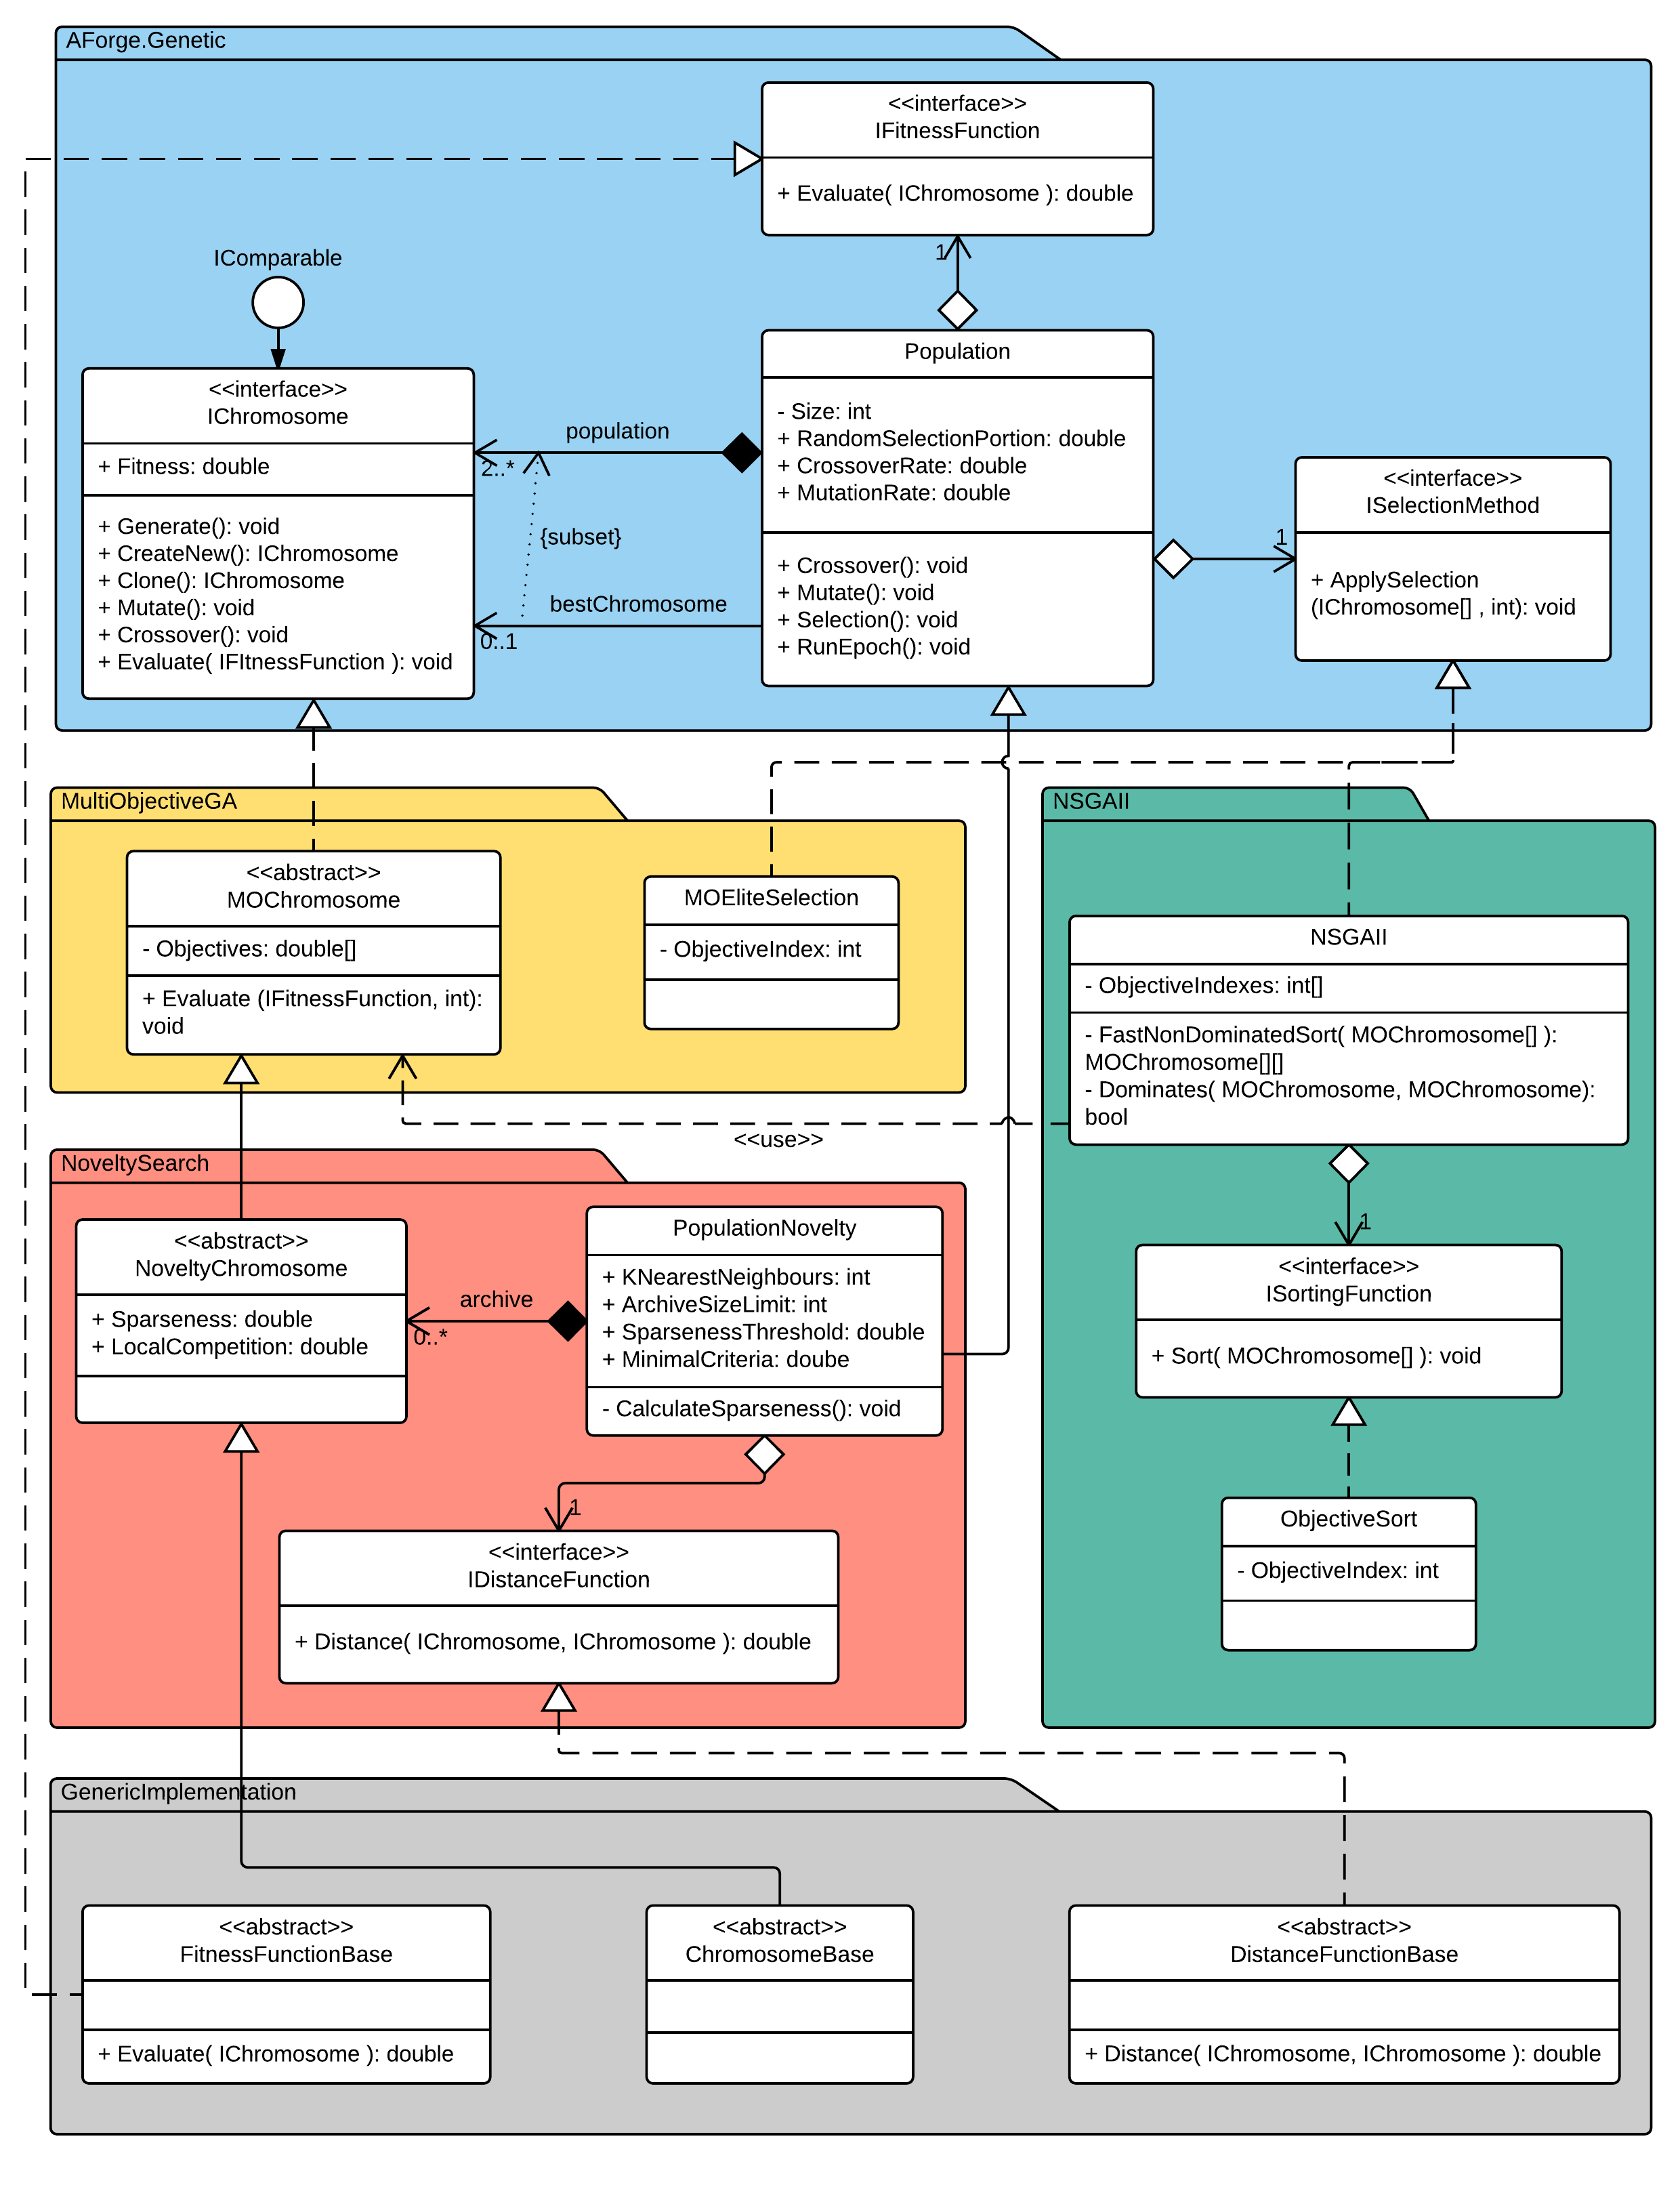
\includegraphics[width=1.0\textwidth]{Imagens/dev_class_diagram.png}
		\caption{Diagrama de Classes do Pacote Computacional.}
		\label{fig:dev_class_diagram}
	\end{center}
\end{figure}

\FloatBarrier

\subsection{Pacote AForge.Genetic}

A implementação base do algoritmo genético utilizada nesta pesquisa foi a da AForge.NET \cite{kirillov2013aforge}, uma \emph{framework} de código aberto desenvolvida em C\# para desenvolvedores e pesquisadores nas áreas de Visão Computacional e Inteligência Artificial. A AForge.NET Framework foi escolhida por possuir o código aberto e de fácil modificação; é escrito de forma modular e bastante organizada possibilitando a extensão para as técnicas utilizadas nesta pesquisa.

Pela forma como foi modularizado, o pacote que implementa o algoritmo genético, o AForge.Genetic, foi utilizado tendo sofrido quase nenhuma modificação. As classes e interfaces utilizadas neste pacote são:
\vspace{-5mm}
\begin{itemize}[leftmargin=1.25\parindent]
    \item \textbf{Population:} Principal responsável pela execução dos métodos do algoritmo genético e manutenção dos indivíduos em cada época.
    \item \textbf{IChromosome:} Interface para a implementação de cromossomos básicos a serem utilizados no algoritmo.
    \item \textbf{IFitnessFunction:} Interface para implementação da função de avaliação.
    \item \textbf{ISelectionMethod:} Interface para implementação do método de seleção que utilizado durante a execução o algoritmo genético.
\end{itemize}

\subsection{Pacote MultiObjectiveGA}

O pacote MultiObjectiveGA tem como função estender as funções implementadas pela AForge.NET Framework à MOEAs, dando suporte à cromossomos com mais de um valor de objetivo. Nesta pesquisa o algoritmo NSGA-II mantém dois valores de objetivo: a dispersão e o valor de competição local. Mesmo na NS pura é desejável e comum se manter tanto o valor de dispersão quanto o valor da função de avaliação como valores de objetivo.

Este pacote é dependente do pacote AForge.Genetic e possui duas classes:
\vspace{-5mm}
\begin{itemize}[leftmargin=1.25\parindent]
    \item \textbf{MOChromosome:} Classe abstrata que implementa a interface \emph{IChromosome} do pacote AForge.Genetic e estende sua performance dando suporte à múltiplos valores de objetivo.
    \item \textbf{MOEliteSelection:} Implementação da interface \emph{ISelectionMethod} do pacote AForge.Genetic, que realiza a seleção elitista com base em um dos objetivos previamente especificado.
\end{itemize}

\subsection{Pacote NSGAII}

O pacote NSGAII possui as classes responsáveis pela implementação do MOEA NSGA-II, dando suporte também à substituição da função de distância de aglomeração, possibilitando a modificação proposta para esta função.

O pacote NSGAII é dependente do Pacote MultiObjectiveGA. São parte deste pacote as seguintes classes e interfaces:
\vspace{-5mm}
\begin{itemize}[leftmargin=1.25\parindent]
    \item \textbf{NSGAII:} Principal classe de implementação do NSGA-II, que classifica e seleciona os melhores indivíduos com base na frente Pareto ótima, calculada em relação aos objetivos analisados em questão.
    \item \textbf{ISortingFunction:} Interface que expõe a implementação do método de ordenação dentro de uma mesma frente não dominada, originalmente a função de distância de aglomeração.
    \item \textbf{ObjectiveSort:} Implementação da interface \emph{ISortingFunction}, que ordena indivíduos dentro de uma mesma frente não dominada com base em um dos objetivos do \emph{MOChromosome} previamente selecionado. Para a metodologia sugerida utilizou-se o valor de dispersão como objetivo para ordenação.
\end{itemize}

\subsection{Pacote NoveltySearch}

O pacote NoveltySearch estende e implementa as classes e interfaces necessárias para realização da PMCNS, adicionando suporte ao cálculo de dispersão, manutenção de um arquivo de indivíduos previamente inovadores e expondo variáveis de controle do algoritmo.

Este pacote é dependente dos pacotes AForge.Genetic e MultiObjectiveGA. São parte deste pacote as seguinte classes e interfaces:
\vspace{-5mm}
\begin{itemize}[leftmargin=1.25\parindent]
    \item \textbf{PopulationNovelty:} Extensão da classe \emph{Population} pertencente ao pacote AForge.Genetic. Implementa os métodos necessários para alterar o algoritmo genético implementado pela AForge.NET Framework e torná-lo uma PMCNS.
    \item \textbf{NoveltyChromosome:} Classe abstrata que estende a classe \emph{MOChromosome} do pacote MultiObjectiveGA. Cromossomo que dá suporte a nota de avaliação, nota de dispersão e nota de competição local. É utilizado pela classe \emph{PopulationNovelty} para execução do PMCNS.
    \item \textbf{IDistanceFunction:} Interface para implementação da função de distância que é utilizada para o cálculo de dispersão durante a NS.
\end{itemize}

\subsection{Pacote GenericImplementation}

O pacote GenericImplementation contém as classes necessárias para aplicação do sistema no domínio de aplicação escolhido. Para a implementação da solução em qualquer domínio, o único pacote do sistema que deve estendido diretamente é esse, não havendo necessidade de alteração em qualquer outra classe ou interface de outros pacotes. O pacote expõe somente as classes que necessitam serem entendidas e implementadas pelo usuário.

Este pacote é dependente de todos os outros previamente listados e contém três classes abstratas:
\vspace{-5mm}
\begin{itemize}[leftmargin=1.25\parindent]
    \item \textbf{ChromosomeBase:} Classe abstrata que estende a classe \emph{NoveltyChromosome} do pacote NoveltySearch. Deve ser estendida e implementar o cromossomo do problema em questão.
    \item \textbf{FitnessFunctionBase:} Classe abstrata que implementa a interface \emph{IFitnessFunction} do pacote AForge.Genetic. Deve ser estendida e implementar a Função de Avaliação responsável por mensurar a qualidade dos indivíduos dentro do contexto definido.
    \item \textbf{DistanceFunctionBase:} Classe abstrata que implementa a interface \emph{IDistanceFunction} do pacote NoveltySearch. Deve ser estendida e implementar a função de distância que delimita o contexto dos nichos da busca.
\end{itemize}

\subsection{Pacote MapEvolution}

A Figura \ref{fig:dev_map_evolution_class_diagram} a seguir apresenta o diagrama de classes para o pacote MapEvolution.

\begin{figure}[htb]
	\begin{center}
		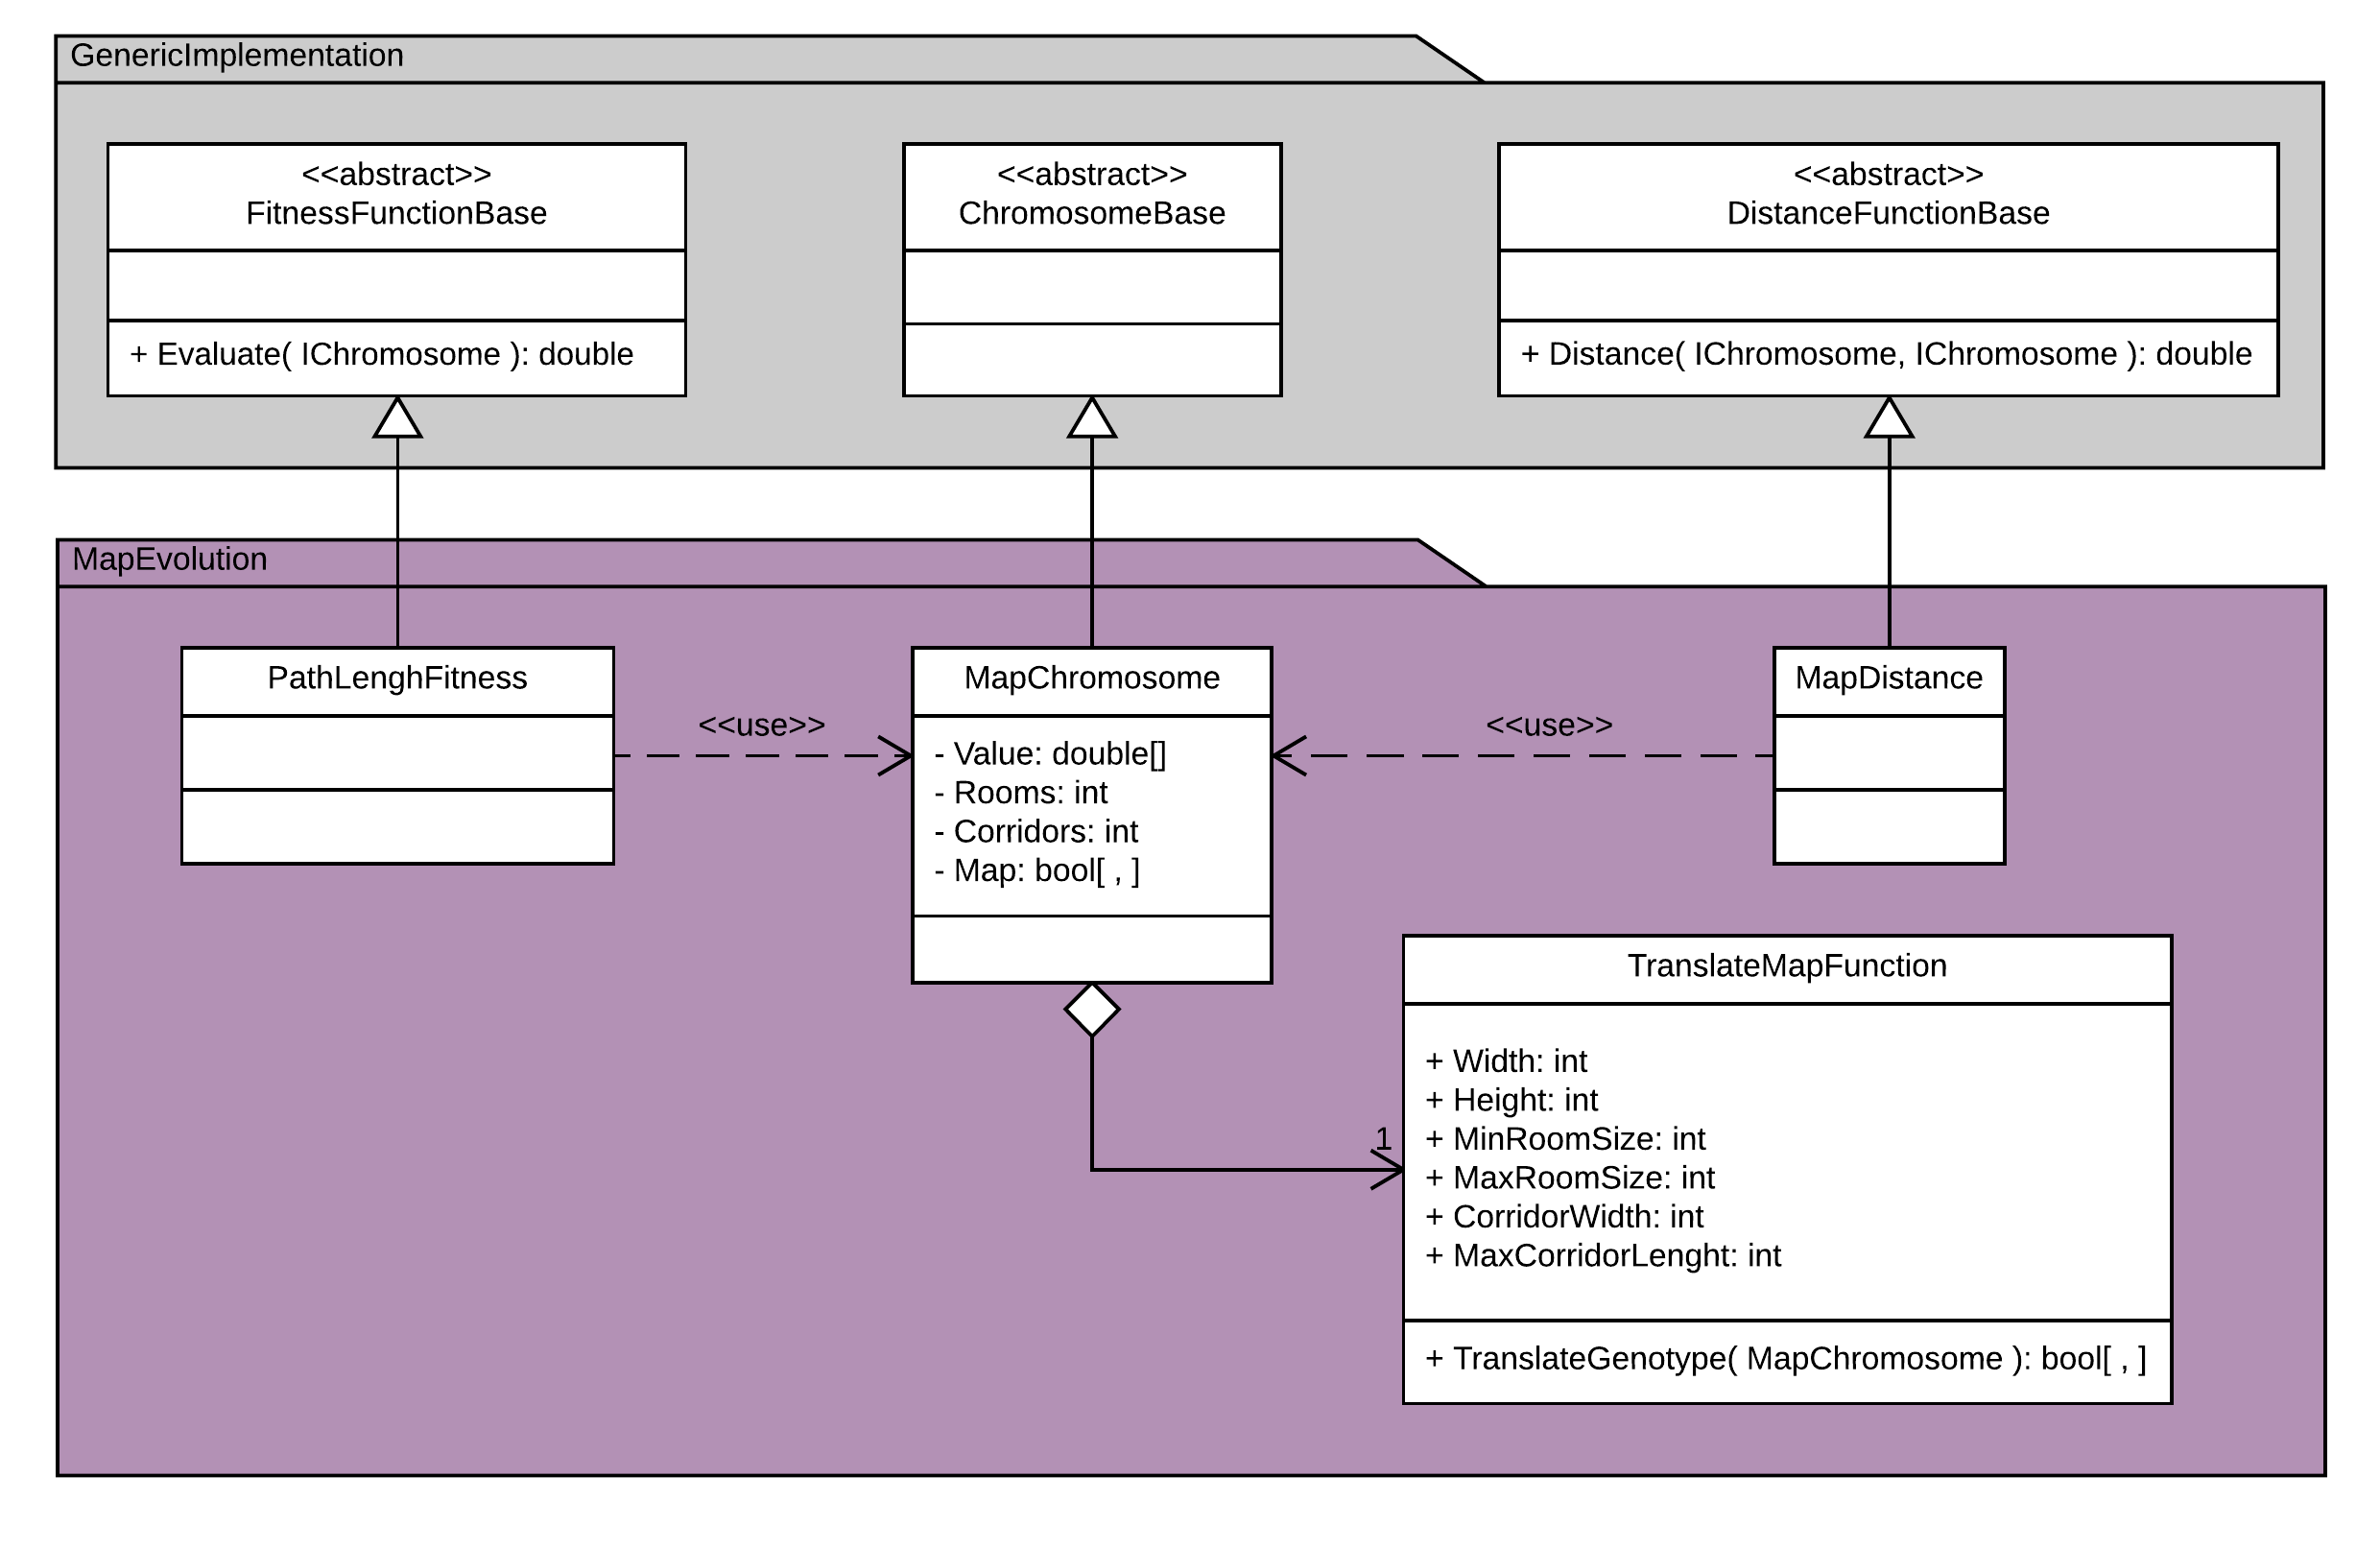
\includegraphics[width=1.0\textwidth]{Imagens/dev_map_evolution_class_diagram.png}
		\caption{Diagrama de Classes do pacote MapEvolution, extendendo as classes abstratas do pacote GenericImplementation.}
		\label{fig:dev_map_evolution_class_diagram}
	\end{center}
\end{figure}

O pacote contém as classes necessárias para aplicação do sistema no contexto de geração de mapas diferenciados para um jogo de aventura. Tipicamente para a utilização do sistema em um domínio específico, se faz necessária a criação de um cromossomo, da função de avaliação e da função de distância já expostas pelo pacote GenericImplementation.

São parte deste pacote as seguinte classes:
\vspace{-5mm}
\begin{itemize}[leftmargin=1.25\parindent]
    \item \textbf{MapChromosome:} Cromossomo utilizado para descrever mapas de um jogo de aventura. Possui informações relacionadas ao genótipo e fenótipo dos mapas evoluídos, assim como seus métodos de troca genética.
    \item \textbf{TranslateMapFunction:} Classe responsável pela tradução de um genótipo de mapa para seu respectivo fenótipo, baseando-se nas variáveis de controle estabelecidas.
    \item \textbf{PathLenghFitness:} Extensão da classe \emph{FitnessFunctionBase} do pacote GenericImplementation, que calcula a nota de avaliação de um mapa ba\-se\-an\-do-se em seu fenótipo, utilizando o cálculo de menor caminho para o mesmo.
    \item \textbf{MapDistance:} Extensão da classe \emph{DistanceFunctionBase} do pacote GenericImplementation, que calcula a distância entre dois mapas dentro do espaço de busca escolhido para a avaliação.
\end{itemize}